\documentclass[8pt]{article}
% Эта строка — комментарий, она не будет показана в выходном файле
\usepackage{ucs}
\usepackage[utf8x]{inputenc} % Включаем поддержку UTF8
\usepackage[russian]{babel}  % Включаем пакет для поддержки русского языка
\usepackage{amsmath}
\usepackage{mathtools}
\usepackage{amssymb}
% \usepackage[dvips]{graphicx}
% \graphicspath{{noiseimages/}}
\usepackage[pdftex]{graphicx}


% Параметры страницы: 1см от правого края и 2см от остальных.


\hoffset=0mm
\voffset=0mm
\textwidth=180mm        % ширина текста
\oddsidemargin=-6.5mm   % левое поле 25.4 - 5.4 = 20 мм
\textheight=240mm       % высота текста 297 (A4) - 40
\topmargin=-15.4mm      % верхнее поле (10мм)
\headheight=5mm      % место для колонтитула
\headsep=5mm          % отступ после колонтитула
\footskip=8mm         % отступ до нижнего колонтитула


\begin{document}
    \author {Зотов Алексей 496 гр.}
    \title {Лабораторная работа 1.5 \\  Изучение колебаний струны}
    \maketitle{}   

    \textbf{Цель работы:} изучение поперечных стоячих волн в струне: определение собственных частот колебания струны в зависимости от натяжения струны и определение скорости распространения поперечных волн в струне. 

    Ограниченная, закрепленная на концах струна, может совершать собственные колебания, представляющие собой стоячие волны вида:
    \begin{equation}
        y(x,t) = A\sin \left (2 \pi f t \right )\sin \left(\frac{2\pi}{\lambda}x \right)
    \end{equation}

    где $A$— амплитуда колебаний в пучностях, $f$ — частота, $\lambda$ — длина волны, $x$ — координата вдоль струны. В концевых точках должны располагаться узлы стоячей волны (амплитуда колебаний равна нулю), откуда следует, что на струне длиной $L$ должно укладываться целое число полуволн:
    \begin{equation}
        L = n \frac{\lambda_n}{2}, \quad n = 1,2,3\dots        
    \end{equation}

    Скорость распространения поперечных волн $u$ зависит от силы натяжения струны $F$ и массы струны на единицу длины 
    $\rho _l$ погонной плотности струны $\rho _l  = \rho S$):
    \begin{equation}
        u = \sqrt{\frac{F}{\rho_l}}
    \end{equation}

    Возможные частоты собственных колебаний струны (обертоны):
    \begin{equation}
        f_n = \frac{u}{\lambda_n} = \frac{n}{2L}\sqrt{\frac{F}{\rho_l}} 
    \end{equation}

    Если частота внешней поперечной синусоидальной силы совпадает с какой либо собственной частотой колебания струны, то возникает явление резонанса и образуется синусоидальная стоячая волна.

    \textbf{В работе используются:} звуковои генератор, двухканальный осциллограф, частотомер, набор грузов, станина, с закрепленной на ней струной ($L = 50$ cm) (Рис.1).

    \begin{center} 
        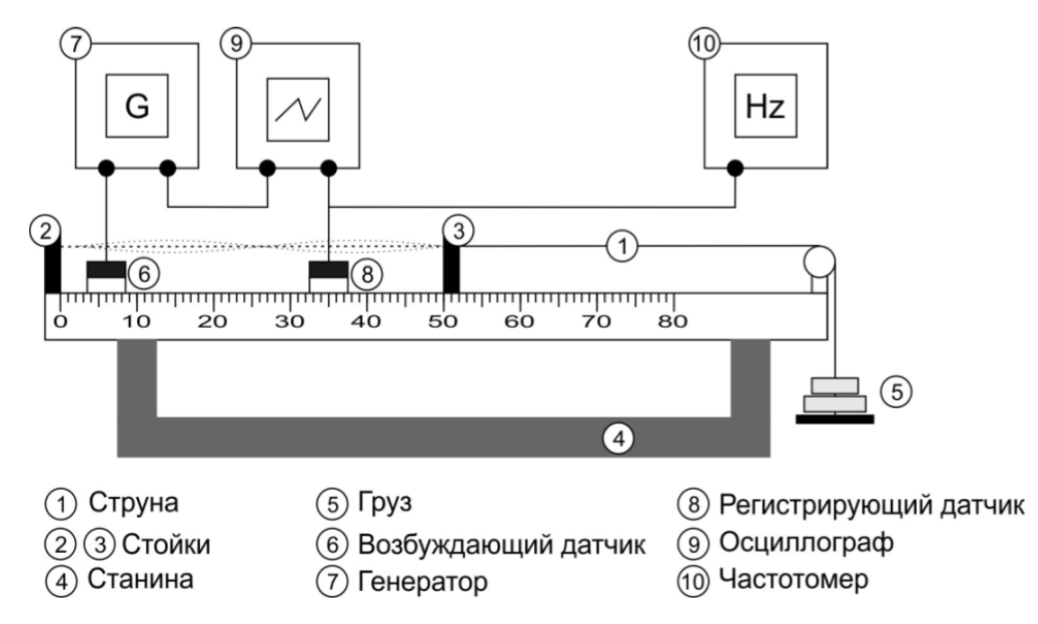
\includegraphics[width=3.5in]{string_img.png} \\ Рис. 1: Экспериментальная установка.
    \end{center}
    
    \textbf{Ход работы:}\\
    \begin{enumerate}
    \item 
         Будем нагружать струну различными массами, и измерять частоты нескольких гармоник стоячих волн.
    Так как ожидаемая зависимость частоты $f\left(n\right)$ линейная, то построим аппроксимирующие по методу наименьших квадратов прямые вида $f = kn + b$ для каждой из нагрузок струны.
    Произведем оценку ошибки:

    \begin{equation}
            \sigma_{k} \approx \frac{1}{\sqrt{n}}
                \sqrt{\frac{\langle y^2 \rangle -  \langle y \rangle ^2}
                        {\langle x^2 \rangle - \langle x \rangle ^2} 
                    - k^2} 
    \end{equation}

    \begin{equation}
            \sigma_{b} = \sigma_{k} \sqrt{\langle x^2 \rangle - \langle x \rangle ^2} 
    \end{equation}

    После этого найдем $u$ - скорость распространения поперечных волн, 
    $f_n = \frac{u}{2L} n \implies u = 2Lk$ , где $k$ - коэффициент наклона прямой $f(n)$ , 
    тогда погрешность определяется как : 
    \begin{equation}
        \left(\frac{\sigma_u}{u} \right)^2 = \left(\frac{\sigma_L}{L}\right)^2 + \left(\frac{\sigma_k}{k}\right)^2
    \end{equation}

    Так как $L$ измерена достаточно точно, то считаем $\sigma_L \approx 0$, тогда $\sigma_k = \sigma_u$
    
    \begin{itemize}
        \item m = 1042.3g
            % \begin{table}[h]
                    % \caption{$\nu(n)$}
                    \begin{center}
                    \begin{tabular}{|c|c|c|c|c|c|c|c|c|}
                            \hline 
                                $n$ & 0 & 1 & 2 & 3 & 4 & 5 & 6 & 7 \\
                            \hline
                                $f_n$ [Гц] &0&127.3&255.7&383.7&512.3&644.2&775.3&904.7\\
                            \hline
                    \end{tabular}
                    \end{center}
            % \end{table}

        \indent $k \approx 129.4$  , $b \approx -2.3$ , $\sigma_k \approx 0.3$ , $\sigma_b \approx 0.6$ , $u \approx 129.4$(м/c) \\
        
        \begin{center} 
            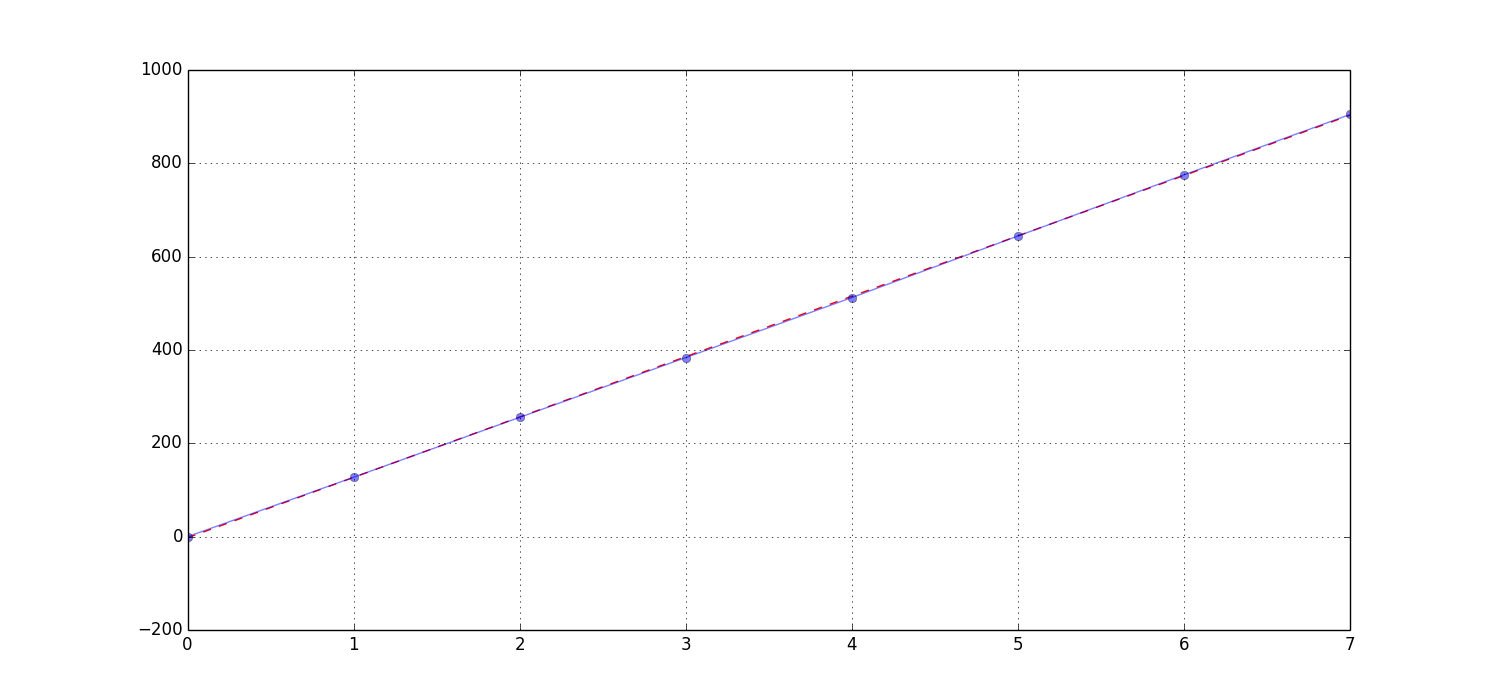
\includegraphics[width=5in]{m0.png} \\ \tiny{$m = 1042.3$}
        \end{center}

        \item m = 548.0g
            % \begin{table}[h]
                    % \caption{$\nu(n)$}
                    \begin{center}
                    \begin{tabular}{|c|c|c|c|c|c|c|}
                            \hline 
                                $n$ & 0 & 1 & 2 & 3 & 4 & 5 \\
                            \hline
                                $f_n$ [Гц] &0&101.1&203.1&303.5&400.0&493.6\\
                            \hline
                    \end{tabular}
                    \end{center}
            % \end{table}
            $k \approx 99.0$  , $b \approx 2.7$ , $\sigma_k \approx 0.7$ , $\sigma_b \approx 1.1$ , $k \approx 99.0$(м/c)\\
            \begin{center} 
                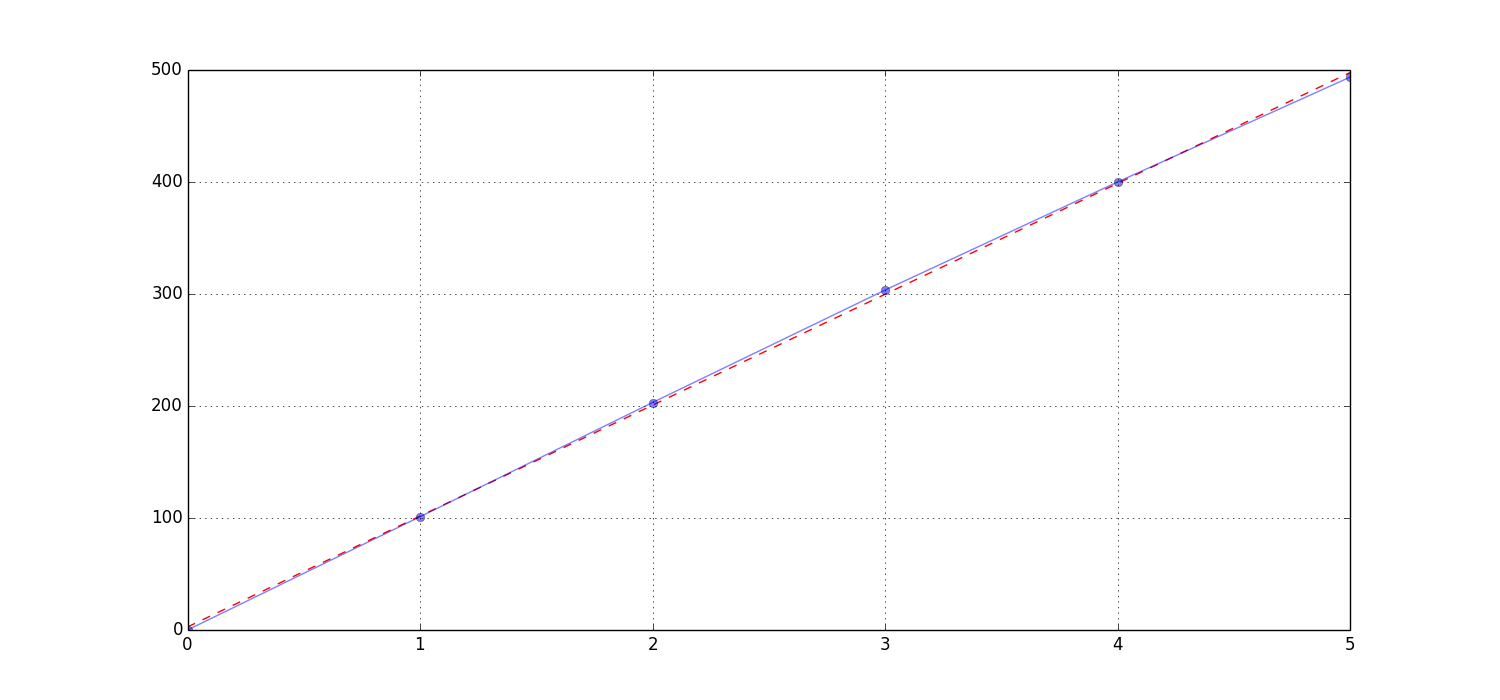
\includegraphics[width=5in]{m1.png} \\ \tiny{$m = 548.0$}
            \end{center}
        \item m = 1544.1g
            % \begin{table}[h]
                    % \caption{$\nu(n)$}
                    \begin{center}
                    \begin{tabular}{|c|c|c|c|c|c|}
                            \hline 
                                $n$ & 0 & 1 & 2 & 3 & 4  \\
                            \hline
                                $f_n$ [Гц] &0&166.0&331.9&498.0&668.1\\
                            \hline
                    \end{tabular}
                    \end{center}
            % \end{table}
            $k \approx 166.8$  , $b \approx -0.8$ , $\sigma_k \approx 0.4$ , $\sigma_b \approx 0.5$ , $u \approx 166.8$(м/c)\\
            \begin{center} 
                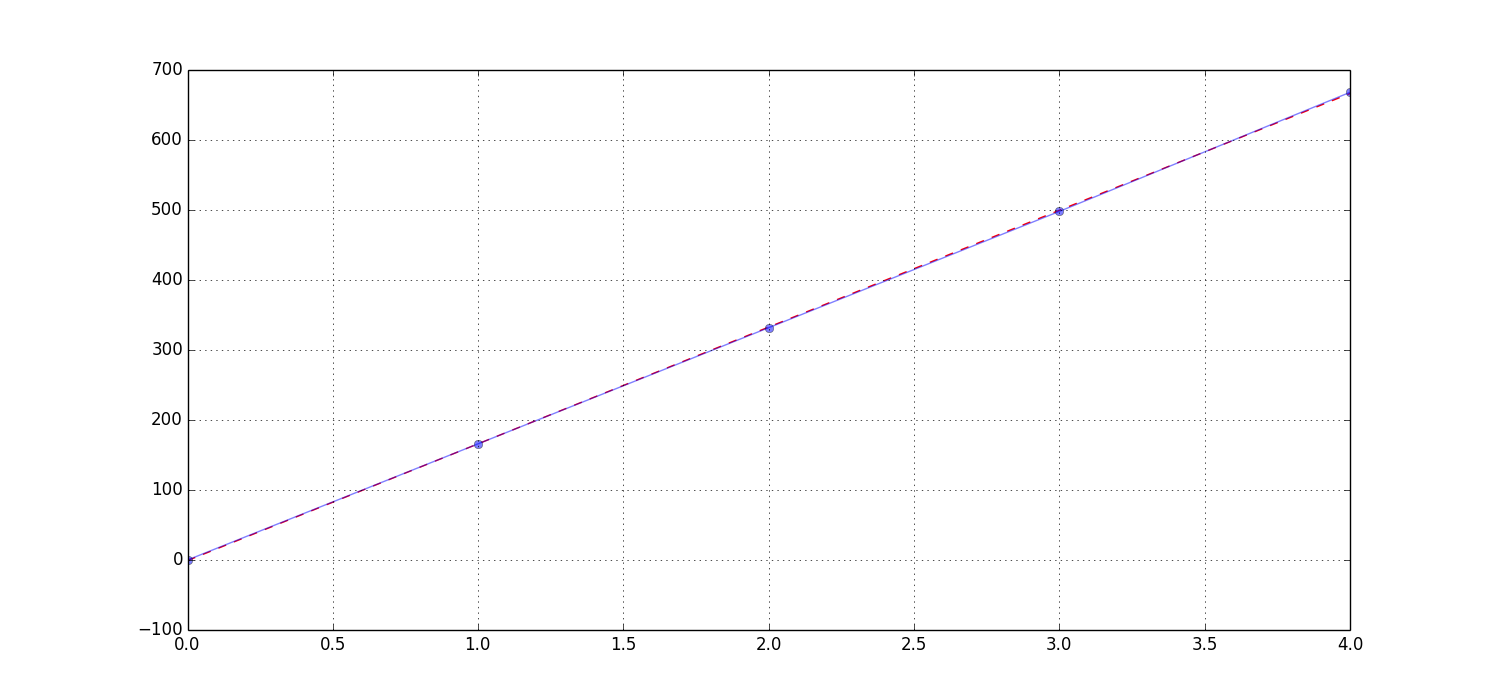
\includegraphics[width=5in]{m2.png} \\ \tiny{$m = 1544.1$}
            \end{center}
        \item m = 2009.0g
            % \begin{table}[h]
                    % \caption{$\nu(n)$}
                    \begin{center}
                    \begin{tabular}{|c|c|c|c|c|c|}
                            \hline 
                                $n$ & 0 & 1 & 2 & 3 & 4  \\
                            \hline
                                $f_n$ [Гц] &0&170.5&341.4&516.9&687.0\\
                            \hline
                    \end{tabular}
                    \end{center}
            % \end{table}
            $k \approx 172.0$  , $b \approx -0.9$ , $\sigma_k \approx 0.4 $ , $\sigma_b \approx 0.5$ , $u \approx 172.0$(м/c)\\
            \begin{center} 
                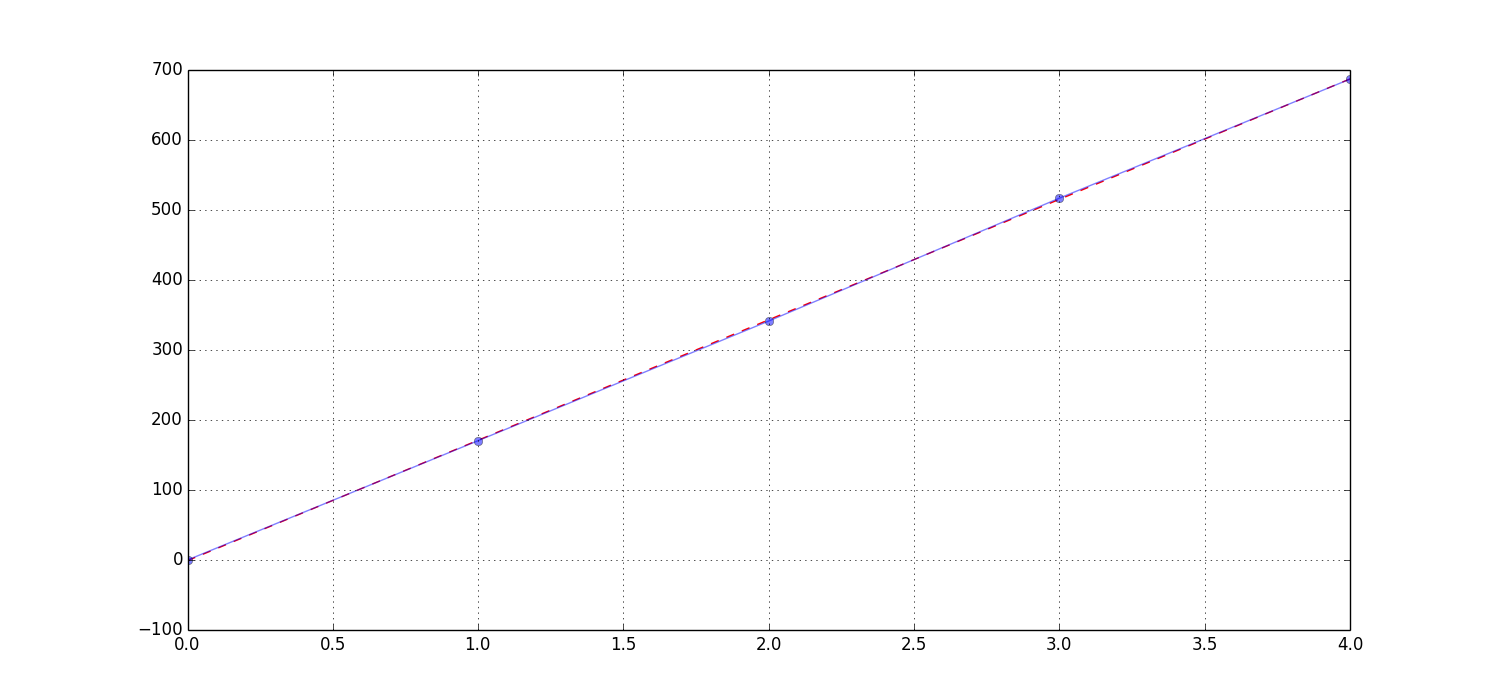
\includegraphics[width=5in]{m3.png} \\\tiny{$m = 2009.0$}
            \end{center}
        \item m = 2514.5g
            % \begin{table}[h]
                    % \caption{$\nu(n)$}
                    \begin{center}
                    \begin{tabular}{|c|c|c|c|c|c|}
                            \hline 
                                $n$ & 0 & 1 & 2 & 3 & 4  \\
                            \hline
                                $f_n$ [Гц] &0&208.7&418.3&629.0&837.1\\
                            \hline
                    \end{tabular}
                    \end{center}
            % \end{table}
            $k \approx 209.5$  , $b \approx -0.3$ , $\sigma_k \approx 0.2$ , $\sigma_b \approx 0.2$ , $u \approx 209.5$(м/c)\\
            \begin{center} 
                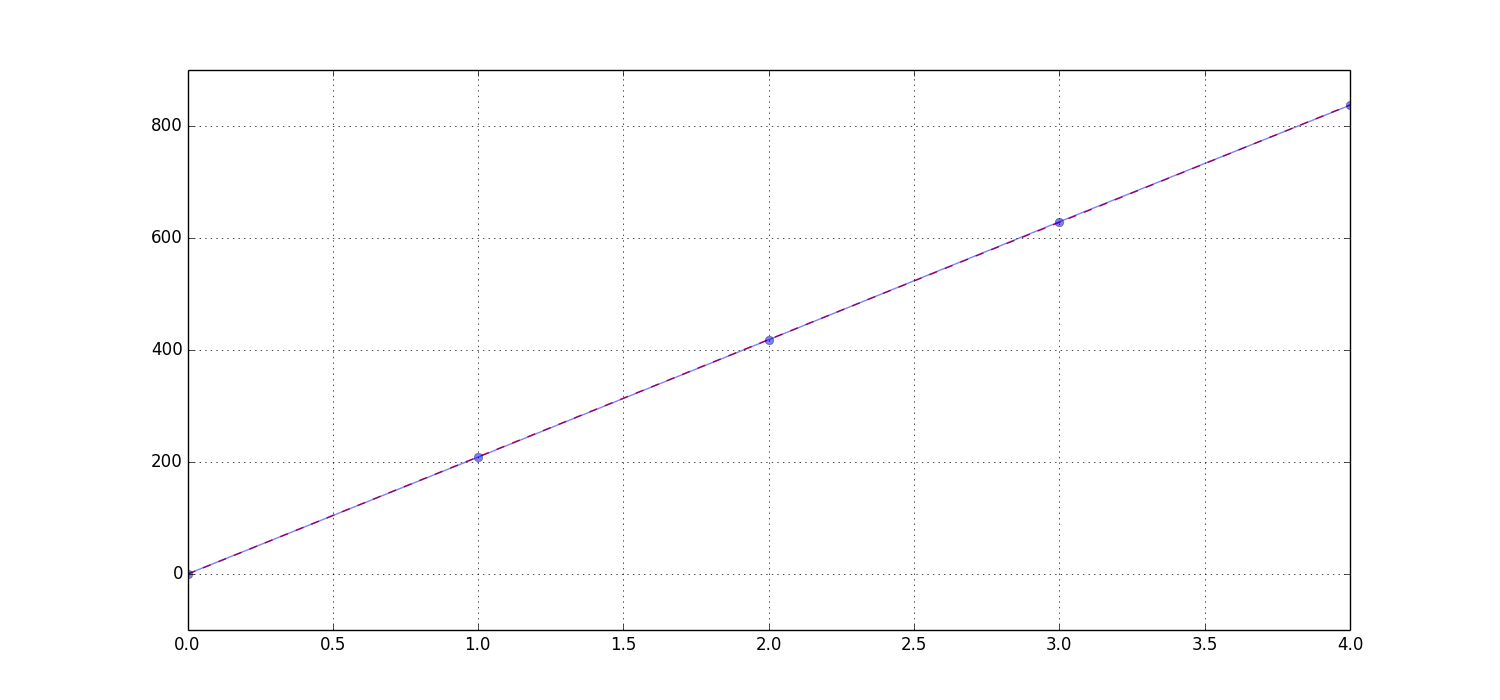
\includegraphics[width=5in]{m4.png} \\ \tiny{$m = 2514.5$}
            \end{center}
    \end{itemize}
    \item
    Найдем зависимость $u^2(F)$ , $F = mg$ , $g \approx 9.81$, $\sigma_u \approx 0.5$, тогда $\sigma_u^2 = 2u \sigma_u \approx 129.4$
    \begin{center} 
                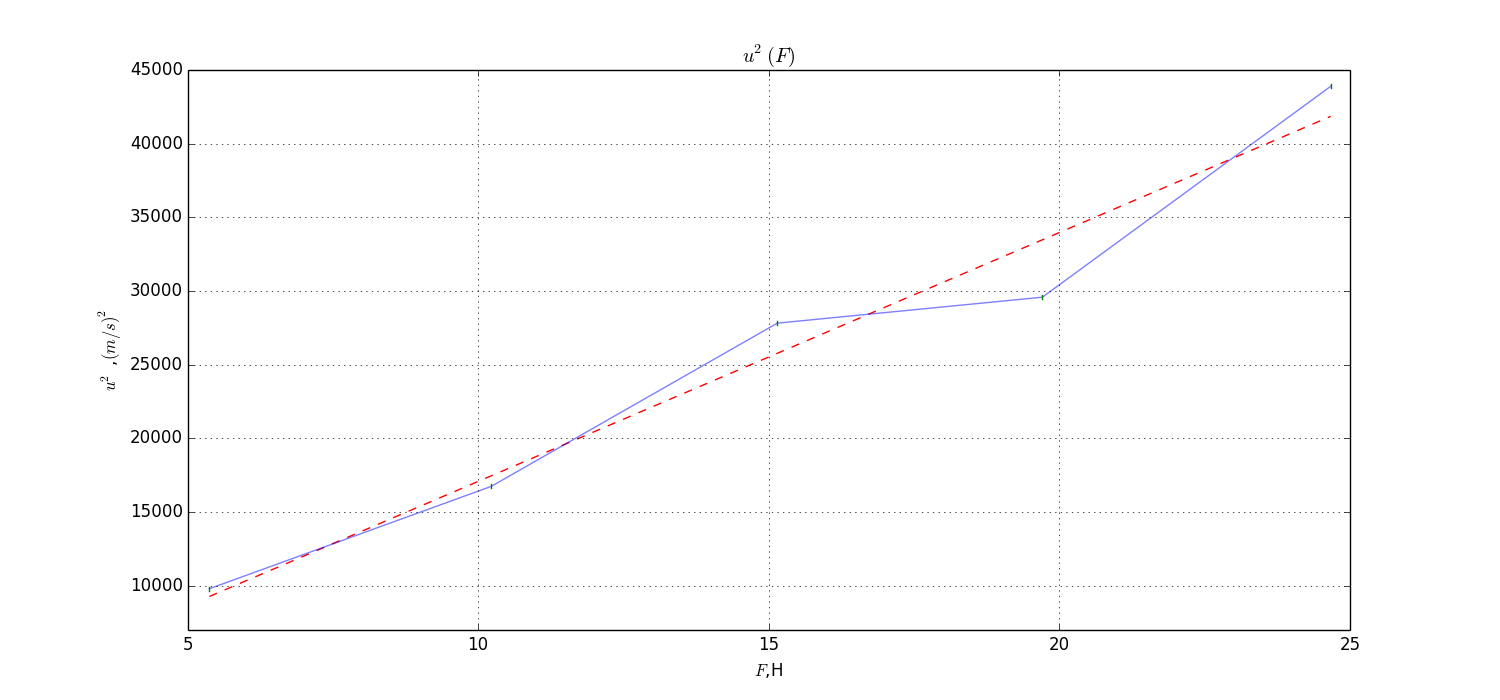
\includegraphics[width=5in]{u2.png} 
    \end{center}
    $y \approx 1688.9 x + 193.3$ , $\sigma_k \approx 145.0$ , $\sigma_b \approx 985.8$
    \item Найдем погонную плотность струны
    \begin{equation}
        \rho_l = \frac{F}{u^2} = 1 / k
    \end{equation}
    $\rho_l \approx 0.59$ [g/m] , 
    $\sigma_{\rho_l} = \frac{1}{k^2} \sigma_k \approx 0.05$ \\
    \item
       Указанная погонная плотность $\rho_{l_0} = 0.5684$ , значит разность ожидаемого и полученного значений укладывается в пределы погрешности.
\end{enumerate}
\end{document}